\documentclass[a4paper]{article}
\usepackage[margin=1in]{geometry}
\usepackage[english]{babel}
\usepackage[utf8]{inputenc}
\usepackage{amsmath}
\usepackage{graphicx}
\usepackage{booktabs}
% \usepackage[colorinlistoftodos]{todonotes}
\usepackage{setspace}
\doublespacing

\title{CAPP 30254: Assignment 1 Write-up}

\author{Daniel Roberts}

\date{\today}

\begin{document}
\maketitle

\section{Problem A}
\begin{enumerate}
\item
\par
First, we have a table of summary statistics. Standard deviation is indicated by "std". The median is indicated by "50\%".
\\
\begin{tabular}{lrrrr}
\toprule
{} &           ID &         Age &         GPA &  Days missed \\
\midrule
count &  1000.000000 &  771.000000 &  779.000000 &   808.000000 \\
mean  &   500.500000 &   16.996109 &    2.988447 &    18.011139 \\
std   &   288.819436 &    1.458067 &    0.818249 &     9.629371 \\
min   &     1.000000 &   15.000000 &    2.000000 &     2.000000 \\
25\%   &   250.750000 &   16.000000 &    2.000000 &     9.000000 \\
50\%   &   500.500000 &   17.000000 &    3.000000 &    18.000000 \\
75\%   &   750.250000 &   18.000000 &    4.000000 &    27.000000 \\
max   &  1000.000000 &   19.000000 &    4.000000 &    34.000000 \\
\bottomrule
\end{tabular}
\\
\par
Below is the table of modes. ID is blank because it is an index variable. Days missed has three entries because the three values are co-modes.
\\
\par
\begin{tabular}{lrllllrrrl}
\toprule
{} &  ID & First\_name & Last\_name &  State &  Gender &  Age &  GPA &  Days missed & Graduated \\
\midrule
 &  &        Amy &      Ross &  Texas &  Female &   15 &    2 &            6 &       Yes \\
 &  &         &        &     &      &   &   &           14 &        \\
 &  &         &        &     &      &   &   &           31 &        \\
\bottomrule
\end{tabular}
\\
\par
Below is the table of missing values.
\\
\par
\begin{tabular}{lrllllrrrl}
\toprule
{} &  ID & First\_name & Last\_name &  State &  Gender &  Age &  GPA &  Days\_missed & Graduated \\
\midrule
& 0 &  0 & 0 & 116 & 226 & 229 & 221 & 192 & 0 \\
\bottomrule
\end{tabular}
\\
\par  
Below are a series of histograms indicating the distributions of numeric variables (age, days missed, GPA) and bar charts indicating frequencies of categorical variables (Gender, Graduation status, and state of origin).
\begin{center}
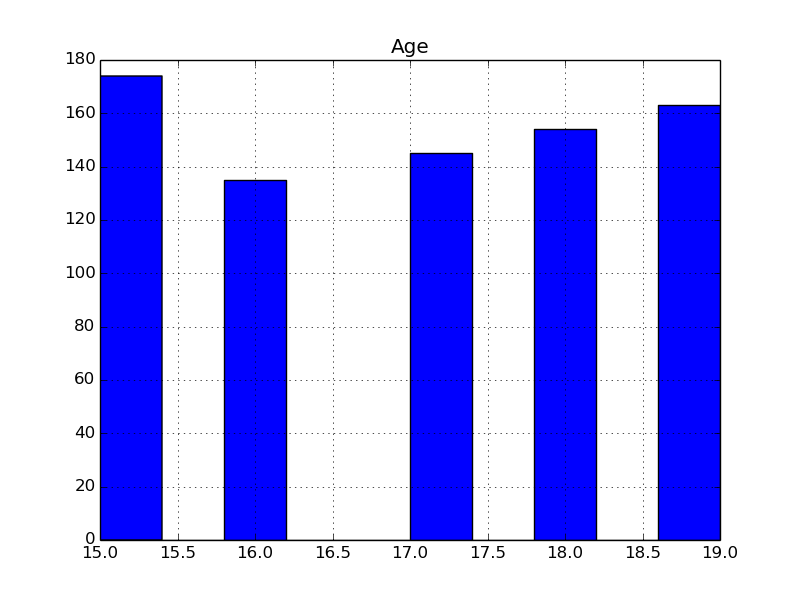
\includegraphics[width=.7\textwidth]{../graphics/Age.png}
\\
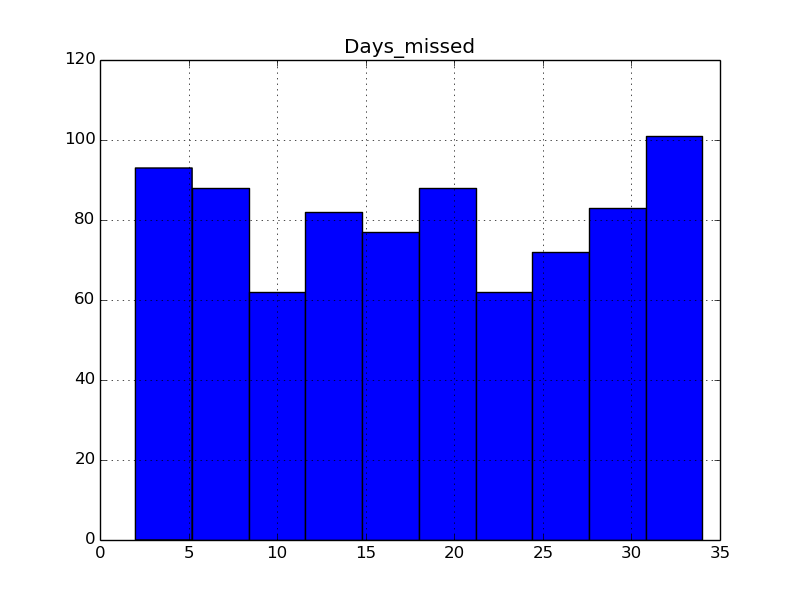
\includegraphics[width=.7\textwidth]{../graphics/Days_missed.png}
\\
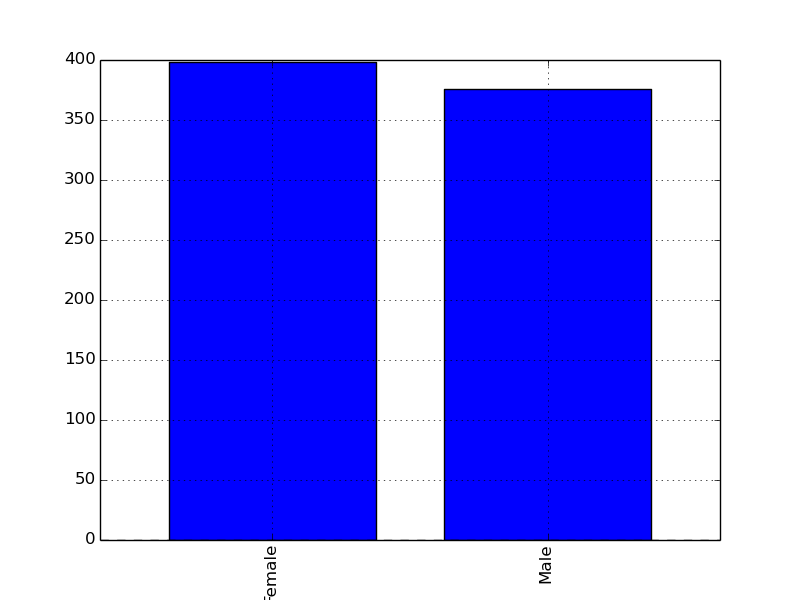
\includegraphics[width=.7\textwidth]{../graphics/Gender.png}
\\
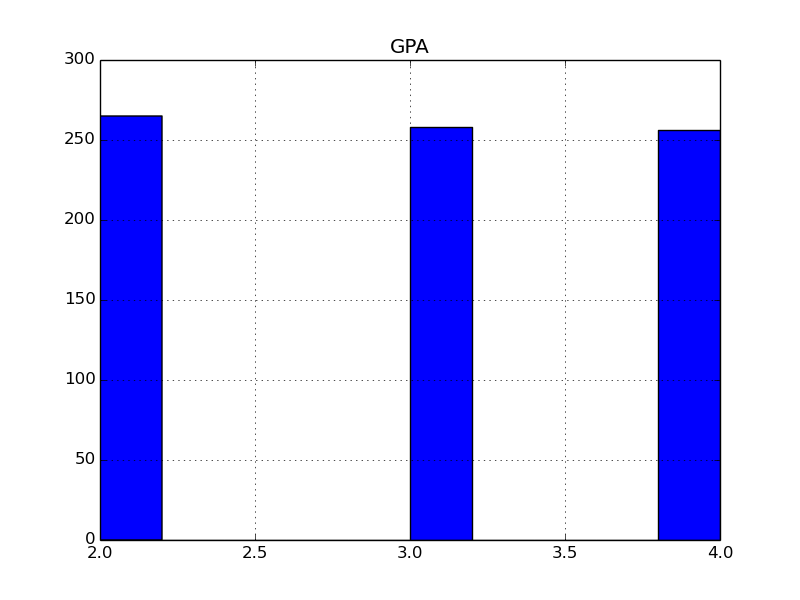
\includegraphics[width=.7\textwidth]{../graphics/GPA.png}
\\
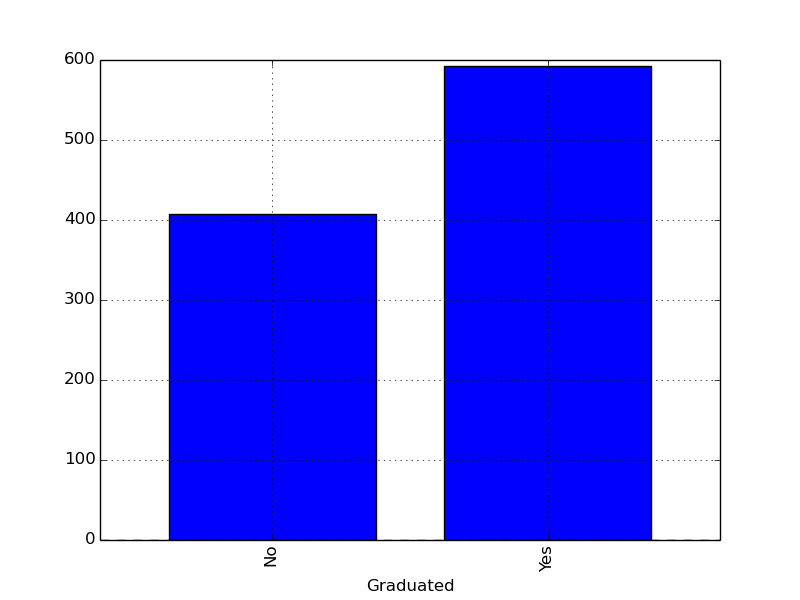
\includegraphics[width=.7\textwidth]{../graphics/Graduated.png}
\\
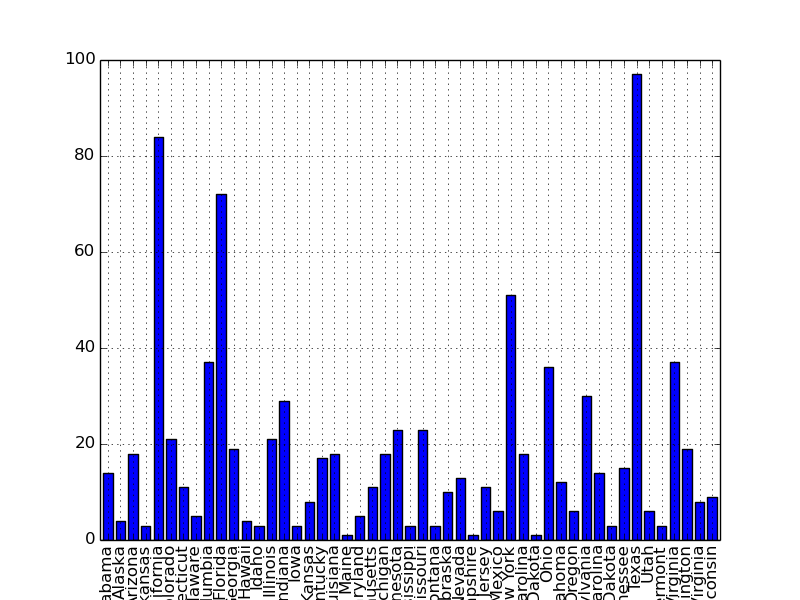
\includegraphics[width=.7\textwidth]{../graphics/State.png}
\\
\end{center}

\newpage

\item
An online API was used to approximate the gender where values were missing by looking at the probability that a given first name was a male or a female name. The interpolated data is stored in the file "gender\_fill\_data.csv" in the repository "dataoutput".

\item

\begin{itemize}
\item 
The missing values were created using the categorical means. The interpolated data is stored in the file "A.csv" in the repository "dataoutput".
\item
The missing values were created using categorical means conditional on graduation. The interpolated data is stored in the file "B.csv" in the repository "dataoutput".
\item
The missing values were created using categorical means conditional on not only graduation, but gender and state as well. By including more seemingly relevant categories over which to group means, we hope to capture more information that would help infer the missing values. The interpolated data is stored in the file "C.csv" in the repository "dataoutput".

\end{itemize}

\end{enumerate}

\section{Problem B}
\begin{enumerate}
\item
Based on the coefficients above, Chris has the higher probability of graduating. First, notice that in our coefficient table, there is a negative coefficient associated with natural log of family income. This implies that a lower income is associated with a higher probability of graduation. Although Chris and David's income are equally below their identical counterparts in absolute terms, Chris' difference (50,000-40,000) is larger in log terms. Thus, we can say that Chris has a higher probability of graduating.
\item
\begin{itemize}
\item
The negative coefficient for AfAm\_Male being negative indicates that all other things being equal, being an African American Male indicates a lower probability (in log probability over one minus probability terms) of graduation. However, this does not mean that African American Males are more likely to not graduate than African-American females. To see this, we can can add the relevant coefficients for a category to see the strength of the effect for an African American Male: AfAmMale + AfAm + Male = 2.648. By contrast, African American Female: AfAm + Female = -.04. Thus all other things being equal an African American male is more likely to graduate than an African American female. Non African American Males have a coefficient 1.45, which is also less than that of African American Males, indicating that African American Males are more likely to graduate.
\item
The age coefficients indicate that all other things being equal, an older student is less likely to graduate than a younger one. However, the interaction effect Age squared indicates that this effect is decreasing in strength as age increases (concavely decreasing probability of graduation).
\item
Whenever a regression is run, there is a problem of multi-collinearity when the independent variables are not linearly independent. This can increase standard errors and result in estimators that provide an unreliable idea of the actual effects of a given variable as opposed to its colinear variables. For example, in this model it seems unnecessary to include both Male and Female: Since this is a binary category all information would be captured by just including one. The effect from age squared is so small in absolute terms that it doesn't seem necessary, and it's close indistinguishable from zero. A similar argument can be made for age, though to a lesser extent.
\end{itemize}
\end{enumerate}





\end{document}